\documentclass[a4paper,10pt]{article}
\usepackage[top=2cm, left=2.5cm, right=2.5cm, bottom=2cm]{geometry}
\usepackage[cmex10]{amsmath}
\usepackage{graphicx}
\usepackage{gvv-book}
\usepackage{gvv}
\usepackage{textcomp}
\usepackage{multicol}

\begin{document}

\title{2021 - AR : Architecture and Planning Exam}
\author{Puni Aditya - EE25BTECH11046}
\date{15th August, 2025}
\maketitle
Duration: Three Hours \hfill Maximum Marks:100

\begin{enumerate}
    \item \begin{itemize}
    \item Arun and Aparna are here.
    \item Arun and Aparna is here.
    \item Arun's families is here.
    \item Arun's family is here.
    Which of the above sentences are grammatically CORRECT? \end{itemize}
    \begin{multicols}{4}
    \begin{enumerate}
        \item (i) and (ii)
        \item (i) and (iv)
        \item (ii) and (iv)
        \item (iii) and (iv)
    \end{enumerate}
    \end{multicols}
    \hfill (GATE-AR 2021)
    
    \item The mirror of the below text about X-axis is \\
    \begin{figure}[h!]
    \centering
    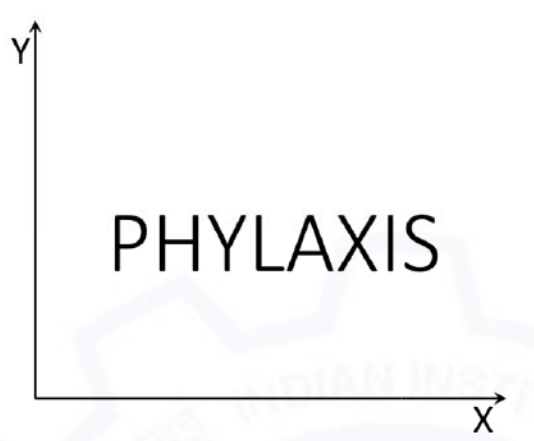
\includegraphics[width=0.3\columnwidth]{figs/01.jpg}
    \caption{}
    \label{fig:Img01}
    \end{figure}
    \begin{enumerate}
    \item \begin{figure}[h!]
    \centering
    
\includegraphics[width=0.1\columnwidth]{figs/02.jpg}
    \caption{}
    \label{fig:Img02}
    \end{figure}
    \item \begin{figure}[h!]
    \centering
    
\includegraphics[width=0.1\columnwidth]{figs/03.jpg}
    \caption{}
    \label{fig:Img03}
    \end{figure}
    \item \begin{figure}[h!]
    \centering
    
\includegraphics[width=0.1\columnwidth]{figs/04.jpg}
    \caption{}
    \label{fig:Img04}
    \end{figure}
    \item \begin{figure}[h!]
    \centering
    
\includegraphics[width=0.1\columnwidth]{figs/05.jpg}
    \caption{}
    \label{fig:Img05}
    \end{figure}
    \end{enumerate}
    
    \item Two identical cube shaped dice each with faces numbered 1 to 6 are rolled simultaneously. The probability that an even number is rolled out on each dice is:
    \begin{multicols}{4}
    \begin{enumerate}
        \item $\frac{1}{36}$
        \item $\frac{1}{12}$
        \item $\frac{1}{8}$
        \item $\frac{1}{4}$
    \end{enumerate}
    \end{multicols}
    \hfill (GATE-AR 2021)

    \item $\oplus$ and $\odot$ are two operators on numbers p and q such that $p \odot q = p - q$, and $p \oplus q = p \times q$. Then, $(9 \odot (6 \oplus 7)) \odot (7 \oplus (6 \odot 5)) =$
    \begin{multicols}{4}
    \begin{enumerate}
        \item 40
        \item -26
        \item -33
        \item -40
    \end{enumerate}
    \end{multicols}
    \hfill (GATE-AR 2021)

    \item Four persons P, Q, R and S are to be seated in a row. R should not be seated at the second position from the left end of the row. The number of distinct seating arrangements possible is:
    \begin{multicols}{4}
    \begin{enumerate}
        \item 6
        \item 9
        \item 18
        \item 24
    \end{enumerate}
    \end{multicols}
    \hfill (GATE-AR 2021)

    \item On a planar field, you travelled 3 units East from a point O. Next you travelled 4 units South to arrive at point P. Then you travelled from P in the North-East direction such that you arrive at a point that is 6 units East of point O. Next, you travelled in the North-West direction, so that you arrive at point Q that is 8 units North of point P. \\
    The distance of point Q to point O, in the same units, should be
    \begin{multicols}{4}
    \begin{enumerate}
        \item 3
        \item 4
        \item 5
        \item 6
    \end{enumerate}
    \end{multicols}
    \hfill (GATE-AR 2021)

    \item The author said, ``Musicians rehearse before their concerts. Actors rehearse their roles before the opening of a new play. On the other hand, I find it strange that many public speakers think they can just walk on to the stage and start speaking. In my opinion, it is no less important for public speakers to rehearse their talks.'' \\
    Based on the above passage, which one of the following is TRUE?
    \begin{enumerate}
        \item The author is of the opinion that rehearsing is important for musicians, actors and public speakers.
        \item The author is of the opinion that rehearsing is less important for public speakers than for musicians and actors.
        \item The author is of the opinion that rehearsing is more important only for musicians than public speakers.
        \item The author is of the opinion that rehearsal is more important for actors than musicians.
    \end{enumerate}
    \hfill (GATE-AR 2021)

    \item 1. Some football players play cricket. \\
    2. All cricket players play hockey. \\
    Among the options given below, the statement that logically follows from the two statements 1 and 2 above, is:
    \begin{enumerate}
        \item No football player plays hockey.
        \item Some football players play hockey.
        \item All football players play hockey.
        \item All hockey players play football.
    \end{enumerate}
    \hfill (GATE-AR 2021)

    \item In the figure shown below, PQRS is a square. The shaded portion is formed by the intersection of sectors of circles with radius equal to the side of the square and centers at S and Q. \\
    The probability that any point picked randomly within the square falls in the shaded area is \\
    \begin{figure}[h!]
    \centering
    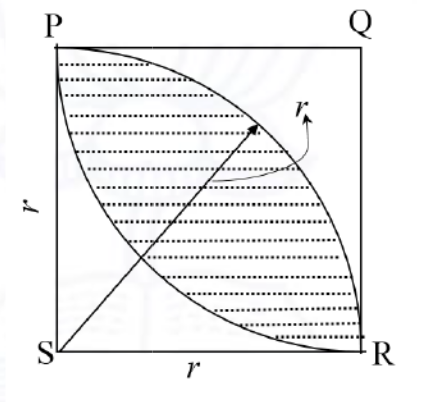
\includegraphics[width=0.5\columnwidth]{figs/06.jpg}
    \caption{Square PQRS}
    \label{fig:Img06}
    \end{figure}
    \begin{multicols}{4}
    \begin{enumerate}
        \item $4 - \frac{\pi}{2}$
        \item $\frac{1}{2}$
        \item $\frac{\pi}{2} - 1$
        \item $\frac{\pi}{4}$
    \end{enumerate}
    \end{multicols}
    \hfill (GATE-AR 2021)

    \item In an equilateral triangle PQR, side PQ is divided into four equal parts, side QR is divided into six equal parts and side PR is divided into eight equal parts. The length of each subdivided part in cm is an integer. The minimum area of the triangle PQR possible, in cm$^2$, is
    \begin{multicols}{4}
    \begin{enumerate}
        \item 18
        \item 24
        \item $48\sqrt{3}$
        \item $144\sqrt{3}$
    \end{enumerate}
    \end{multicols}
    \hfill (GATE-AR 2021)
    
    \item As per National Building Code of India, 2016, the function of an Automatic Rescue Device is to 
    \begin{enumerate}
        \item bring a stuck lift to the nearest landing level.
        \item control fire in electrical system at plenum level.
        \item control the escape route lighting system.
        \item trigger fire sprinkler system.
    \end{enumerate}
    \hfill (GATE-AR 2021)

    \item Which among the following acronyms represents a thermal comfort index? 
    \begin{multicols}{4}
    \begin{enumerate}
        \item PMV
        \item NDVI
        \item DEM
        \item PCA
    \end{enumerate}
    \end{multicols}
    \hfill (GATE-AR 2021)

    \item Indian satellite sensor that can be used for very high resolution mapping of urban areas is 
    \begin{multicols}{2}
    \begin{enumerate}
        \item LANDSAT.
        \item CARTOSAT.
        \item RESOURCESAT.
        \item MODIS.
    \end{enumerate}
    \end{multicols}
    \hfill (GATE-AR 2021)

    \item What is the smallest entity of raster data used in GIS? 
    \begin{multicols}{4}
    \begin{enumerate}
        \item Line
        \item Pixel
        \item Point
        \item Polygon
    \end{enumerate}
    \end{multicols}
    \hfill (GATE-AR 2021)

    \item The correct sequence of stages during firing/burning of bricks is 
    \begin{enumerate}
        \item Dehydration - Oxidation - Vitrification - Cooling.
        \item Vitrification - Dehydration - Oxidation - Cooling.
        \item Oxidation - Dehydration - Vitrification - Cooling.
        \item Cooling - Oxidation - Vitrification - Dehydration.
    \end{enumerate}
    \hfill (GATE-AR 2021)

    \item Industry Foundation Classes (IFC) in BIM is 
    \begin{enumerate}
        \item a module used to improve energy savings.
        \item an algorithm related to the precision of the BIM model.
        \item a program based on Bezier Splines.
        \item an object oriented data model to facilitate interoperability.
    \end{enumerate}
    \hfill (GATE-AR 2021)

    \item As per urban design principles proposed by Gordon Cullen, Rashtrapati Bhavan, New Delhi, is an example of 
    \begin{multicols}{2}
    \begin{enumerate}
        \item Serial Vision.
        \item Pinpointing.
        \item Occupied territory.
        \item Here and there.
    \end{enumerate}
    \end{multicols}
    \hfill (GATE-AR 2021)

    \item A waste water pipe connecting two inspection chambers (IC) is laid at a slope of 1:200. The Invert Level of the starting IC is -450 mm. The Invert level of the second pit at a distance of 40 m from the first IC is 
    \begin{multicols}{4}
    \begin{enumerate}
        \item -650 mm.
        \item -200 mm.
        \item -250 mm.
        \item -550 mm.
    \end{enumerate}
    \end{multicols}
    \hfill (GATE-AR 2021)

    \item From the images P, Q and R given below, select the corresponding land use categories according to Alonso's Bid Rent Theory. \\
    \begin{figure}[h!]
    \centering
    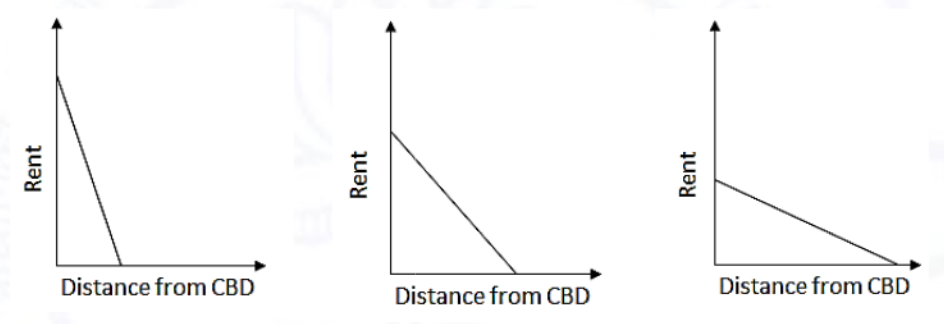
\includegraphics[width=0.5\columnwidth]{figs/07.jpg}
    \caption{Rent vs Distance CBD Graphs}
    \label{fig:Img07}
    \end{figure}
    \begin{enumerate}
        \item P-Manufacturing; Q-Residential; R-Retail
        \item P-Retail; Q-Residential; R-Manufacturing
        \item P-Residential; Q-Retail; R-Manufacturing
        \item P-Retail; Q-Manufacturing; R-Residential
    \end{enumerate}
    \hfill (GATE-AR 2021)

    \item The urban land use model based on the concept of a polycentric city is known as 
    \begin{multicols}{2}
    \begin{enumerate}
        \item Burgess Model.
        \item Harris and Ullman model.
        \item Hagerstrand's Model.
        \item Homer Hoyt's model.
    \end{enumerate}
    \end{multicols}
    \hfill (GATE-AR 2021)

    \item The total head or total lift against which a pump works includes suction lift, discharge lift and 
    \begin{multicols}{2}
    \begin{enumerate}
        \item cone of depression.
        \item salvage lift.
        \item water horse power.
        \item frictional head loss.
    \end{enumerate}
    \end{multicols}
    \hfill (GATE-AR 2021)

    \item The two components for measuring time of concentration for storm water are 
    \begin{enumerate}
        \item overland flow time and retention time.
        \item overland flow time and gutter flow time.
        \item detention time and gutter flow time.
        \item retention time and inlet time.
    \end{enumerate}
    \hfill (GATE-AR 2021)

    \item The traffic assignment technique where the traffic arranges itself in congested networks such that the journey time in all used routes between an Origin-Destination pair are equal and less than those that would be experienced in all unused routes. This is known as 
    \begin{multicols}{2}
    \begin{enumerate}
        \item System equilibrium.
        \item All-or-nothing.
        \item User equilibrium.
        \item Incremental.
    \end{enumerate}
    \end{multicols}
    \hfill (GATE-AR 2021)

    \item What is the dependent variable in a regression based trip generation model? 
    \begin{enumerate}
        \item Population of Traffic Analysis Zone
        \item Number of trips
        \item Number of employees
        \item Number of households
    \end{enumerate}
    \hfill (GATE-AR 2021)

    \item The curve traced by a point on a circle rolling inside another circle is known as 
    \begin{multicols}{4}
    \begin{enumerate}
        \item hypocycloid.
        \item helix.
        \item involute.
        \item hyperbola.
    \end{enumerate}
    \end{multicols}
    \hfill (GATE-AR 2021)

    \item The law of Primate City was first proposed by 
    \begin{multicols}{2}
    \begin{enumerate}
        \item Samuel A. Stouffer.
        \item Colin Clark.
        \item Mark Jefferson.
        \item Harold Hotelling.
    \end{enumerate}
    \end{multicols}
    \hfill (GATE-AR 2021)

    \item In the European Union which constitutes the cities namely, London, Paris, Brussels, Amsterdam, Cologne, Frankfurt, Munich and Milan, lie within a linear megalopolitan zone known as 
    \begin{multicols}{2}
    \begin{enumerate}
        \item Purple Zone.
        \item Golden Polygon.
        \item Blue Banana.
        \item Yellow Corridor.
    \end{enumerate}
    \end{multicols}
    \hfill (GATE-AR 2021)

    \item An urban governance tool to mobilize financial resources by permitting additional FAR over and above the prescribed FAR by imposing a charge or fee for the same is known as 
    \begin{enumerate}
        \item Betterment Levy.
        \item Impact Fee.
        \item Land Value Increment Tax.
        \item Floor Area Incentive Tax.
    \end{enumerate}
    \hfill (GATE-AR 2021)

    \item Identify the colour palette that is created using any three equally spaced hues around the colour wheel. 
    \begin{multicols}{2}
    \begin{enumerate}
        \item Split-complementary
        \item Analogous
        \item Triads
        \item Complementary
    \end{enumerate}
    \end{multicols}
    \hfill (GATE-AR 2021)

    \item Coefficient of Performance (COP) for heat pump is used to calculate 
    \begin{enumerate}
        \item the number of air changes.
        \item the Energy Efficiency Ratio.
        \item the Energy Select Sector index.
        \item the Indoor Air Quality index.
    \end{enumerate}
    \hfill (GATE-AR 2021)

    \item Freight flows are converted to truck flows using 
    \begin{multicols}{2}
    \begin{enumerate}
        \item Volume factor.
        \item Weight factor.
        \item Payload factor.
        \item Distance load factor.
    \end{enumerate}
    \end{multicols}
    \hfill (GATE-AR 2021)

    \item Rebound hammer test is used to measure 
    \begin{enumerate}
        \item permeability of concrete.
        \item bond stress between rebar and concrete.
        \item compressive strength of concrete.
        \item tensile strength of concrete.
    \end{enumerate}
    \hfill (GATE-AR 2021)

    \item Which type of temporary supporting structure can be used in case of rebuilding the lower part of a load bearing wall at ground floor above plinth level? 
    \begin{multicols}{2}
    \begin{enumerate}
        \item Dead Shore
        \item Pit Underpinning
        \item Flying Shore
        \item Needle Scaffolding
    \end{enumerate}
    \end{multicols}
    \hfill (GATE-AR 2021)

    \item During earthquake, soft storey failure in a building is due to 
    \begin{enumerate}
        \item shear failure initiated by short column effect.
        \item stress discontinuity initiated by abrupt changes of stiffness.
        \item failure of column initiated by weak column-strong beam effect.
        \item drift of building storey initiated by pounding effect.
    \end{enumerate}
    \hfill (GATE-AR 2021)

    \item Following five activities are associated with construction contract management. Choose the option showing the correct progressive sequence of the activities. \\
    \begin{tabular}{ l l }
    P & Opening of Bid \\
    Q & Submission of Security Deposit \\
    R & Publication of Notice Inviting Tender (NIT) \\
    S & Issue of Letter of Intent (LOI) \\
    T & Submission of Earnest Money Deposit (EMD) \\
    \end{tabular}
    \begin{multicols}{2}
    \begin{enumerate}
        \item R-Q-P-T-S
        \item S-P-R-T-Q
        \item R-T-P-S-Q
        \item S-T-P-R-Q
    \end{enumerate}
    \end{multicols}
    \hfill (GATE-AR 2021)

    \item Match the acronyms in \textbf{Group I} with the particulars in \textbf{Group II}. \\
    \begin{tabular}{ l l }
    \textbf{Group I} & \textbf{Group II} \\
    P. LCA & 1. building certification system \\
    Q. IPCC & 2. hydrological assessment tool \\
    R. Mtoe & 3. climate change \\
    S. LEED & 4. equivalent measure of energy expended \\
    & 5. cradle to grave \\
    \end{tabular}
    \begin{multicols}{2}
    \begin{enumerate}
        \item P-3, Q-5, R-4, S-2
        \item P-4, Q-3, R-1, S-2
        \item P-5, Q-4, R-2, S-1
        \item P-5, Q-3, R-4, S-1
    \end{enumerate}
    \end{multicols}
    \hfill (GATE-AR 2021)

    \item Match the buildings in \textbf{Group I} with their corresponding architect in \textbf{Group II}. \\
    \begin{figure}[h!]
    \centering
    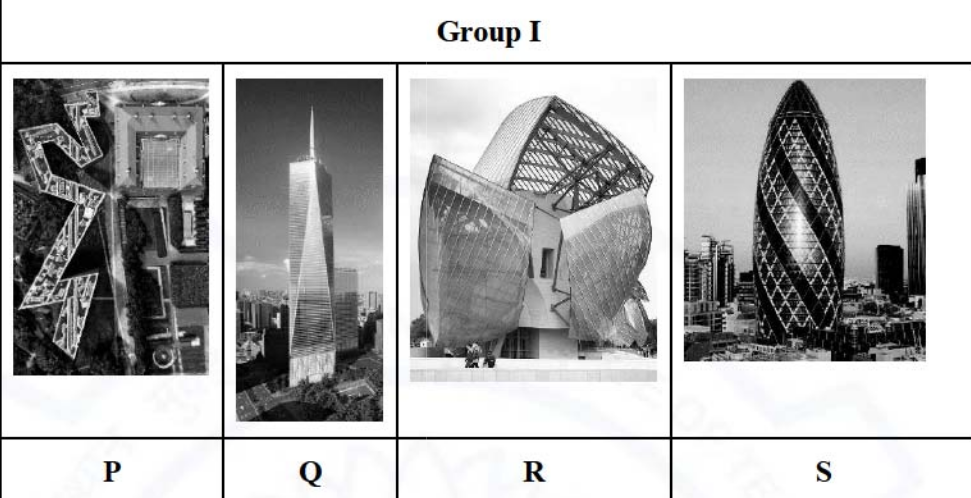
\includegraphics[width=0.5\columnwidth]{figs/08.jpg}
    \caption{Buildings}
    \label{fig:Img08}
    \end{figure} \\
    \textbf{Group II} \\
    1. Renzo Piano \\ 
    2. Daniel Libeskind \\
    3. David Childs \\
    4. Frank Owen Gehry \\
    5. Norman Foster \\
    \begin{multicols}{2}
    \begin{enumerate}
        \item P-4, Q-3, R-1, S-2
        \item P-2, Q-4, R-2, S-5
        \item P-3, Q-5, R-4, S-1
        \item P-3, Q-5, R-1, S-2
    \end{enumerate}
    \end{multicols}
    \hfill (GATE-AR 2021)

    \item Match the heritage conservation charters in \textbf{Group I} with their focus areas in \textbf{Group II}. \\
    \begin{tabular}{ l l }
    \textbf{Group I} & \textbf{Group II} \\
    P. Washington Charter & 1. Conservation of historic gardens \\
    Q. Florence Charter & 2. Conservation of places of cultural significance \\
    R. Venice Charter & 3. Authenticity \\
    S. Burra Charter & 4. Conservation \& restoration of monuments and sites \\
    & 5. Conservation of historic towns \\
    \end{tabular}
    \begin{multicols}{2}
    \begin{enumerate}
        \item P-3, Q-1, R-4, S-5
        \item P-5, Q-4, R-1, S-2
        \item P-5, Q-1, R-4, S-2
        \item P-4, Q-1, R-3, S-2
    \end{enumerate}
    \end{multicols}
    \hfill (GATE-AR 2021)

    \item Match the Buildings (name of architects) in \textbf{Group I} with the abstractions used in \textbf{Group II}. \\
    \begin{tabular}{ l l }
    \textbf{Group I} & \textbf{Group II} \\
    P. The School for Spastic Children, New Delhi (Romi Khosla) & 1. Cosmos in geometric form \\
    Q. Jawahar Kala Kendra, Jaipur (Charles Correa) & 2. Panchavati \\
    R. Capitol Complex, Chandigarh (Le Corbusier) & 3. Plan form of Hindu temple \\
    S. Oberoi Hotel, Bhubaneswar (Satish Grover) & 4. Bull's horns \\
    & 5. Mother's womb \\
    \end{tabular}
    \begin{multicols}{2}
    \begin{enumerate}
        \item P-4, Q-2, R-1, S-3
        \item P-5, Q-1, R-4, S-3
        \item P-2, Q-1, R-3, S-2
        \item P-5, Q-2, R-4, S-1
    \end{enumerate}
    \end{multicols}
    \hfill (GATE-AR 2021)

    \item Match the names of the gardens in \textbf{Group I} with their type in \textbf{Group II}. \\
    \begin{tabular}{ l l }
    \textbf{Group I} & \textbf{Group II} \\
    P. Shalimar Bagh, Srinagar & 1. Hanging Garden \\
    Q. Pherozeshah Mehta Garden, Mumbai & 2. Memorial Garden \\
    R. Lalbagh Garden, Bangalore & 3. Rock Garden \\
    S. Nek Chand's Garden, Chandigarh & 4. Botanical Garden \\
    & 5. Mughal Garden \\
    \end{tabular}
    \begin{multicols}{2}
    \begin{enumerate}
        \item P-3, Q-1, R-2, S-4
        \item P-5, Q-1, R-4, S-3
        \item P-5, Q-3, R-4, S-2
        \item P-5, Q-4, R-1, S-3
    \end{enumerate}
    \end{multicols}
    \hfill (GATE-AR 2021)

    \item Match the various types of impurities present in water in \textbf{Group I} with the appropriate water treatment process given in \textbf{Group II}. \\
    \begin{tabular}{ l l }
    \textbf{Group I} & \textbf{Group II} \\
    P. Fine suspended matter & 1. Aeration \\
    Q. Pathogenic bacteria & 2. Plain sedimentation \\
    R. Color, odour and taste & 3. Sedimentation with coagulation \\
    S. Floating matter as leaves & 4. Screening \\
    & 5. Disinfection \\
    \end{tabular}
    \begin{multicols}{2}
    \begin{enumerate}
        \item P-2, Q-5, R-3, S-4
        \item P-3, Q-4, R-1, S-2
        \item P-1, Q-4, R-3, S-2
        \item P-3, Q-5, R-1, S-4
    \end{enumerate}
    \end{multicols}
    \hfill (GATE-AR 2021)

    \item Match the temples in \textbf{Group I} with their style of Architecture in \textbf{Group II} \\
    \begin{tabular}{ l l }
    \textbf{Group I} & \textbf{Group II} \\
    P. Badami Cave Temples & 1. Pandya style \\
    Q. Kalugumalai Temple Complex & 2. Chola style \\
    R. Airavatesvara Temple & 3. Chalukya style \\
    S. Chennakeshava Temple & 4. Vijayanagara style \\
    & 5. Hoysala style \\
    \end{tabular}
    \begin{multicols}{2}
    \begin{enumerate}
        \item P-3, Q-1, R-2, S-5
        \item P-3, Q-4, R-2, S-1
        \item P-2, Q-1, R-3, S-5
        \item P-5, Q-1, R-4, S-2
    \end{enumerate}
    \end{multicols}
    \hfill (GATE-AR 2021)

    \item Match the urban form/structure in \textbf{Group I} with their respective proponents in \textbf{Group II}. \\
    \begin{tabular}{ l l }
    \textbf{Group I} & \textbf{Group II} \\
    P. Trabantenstadte & 1. Arturo Soria Y Mata \\
    Q. Linear city & 2. Le Corbusier \\
    R. Bloomsbury Precinct & 3. Ernst May \\
    S. Radiant city & 4. Frank Lloyd Wright \\
    & 5. Patrick Abercrombie \\
    \end{tabular}
    \begin{multicols}{2}
    \begin{enumerate}
        \item P-4, Q-1, R-5, S-3
        \item P-5, Q-1, R-4, S-2
        \item P-3, Q-1, R-5, S-2
        \item P-3, Q-4, R-1, S-2
    \end{enumerate}
    \end{multicols}
    \hfill (GATE-AR 2021)

    \item Match the elements in \textbf{Group I} to their description in \textbf{Group II}. \\
    \textbf{Group I}
    \begin{figure}[h!]
    \centering
    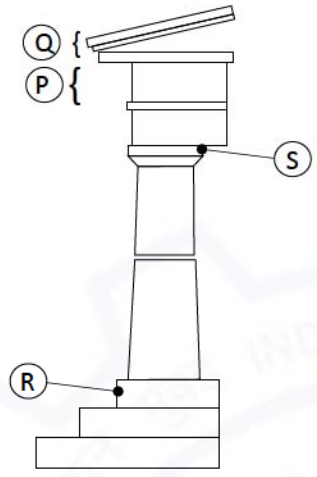
\includegraphics[width=0.25\columnwidth]{figs/09.jpg}
    \caption{}
    \label{fig:Img09}
    \end{figure}
    \newpage
    \textbf{Group II} \\
    1. Cornice \\
    2. Stylobate \\
    3. Stereobate \\
    4. Abacus \\
    5. Frieze \\
    \begin{multicols}{2}
    \begin{enumerate}
        \item P-3, Q-1, R-5, S-4
        \item P-4, Q-3, R-1, S-2
        \item P-5, Q-4, R-2, S-1
        \item P-5, Q-1, R-2, S-4
    \end{enumerate}
    \end{multicols}
    \hfill (GATE-AR 2021)

    \item Match the position of feet in \textbf{Group I} to the most appropriate description of stability of human body in \textbf{Group II}. \\
	    \begin{figure}[h!]
    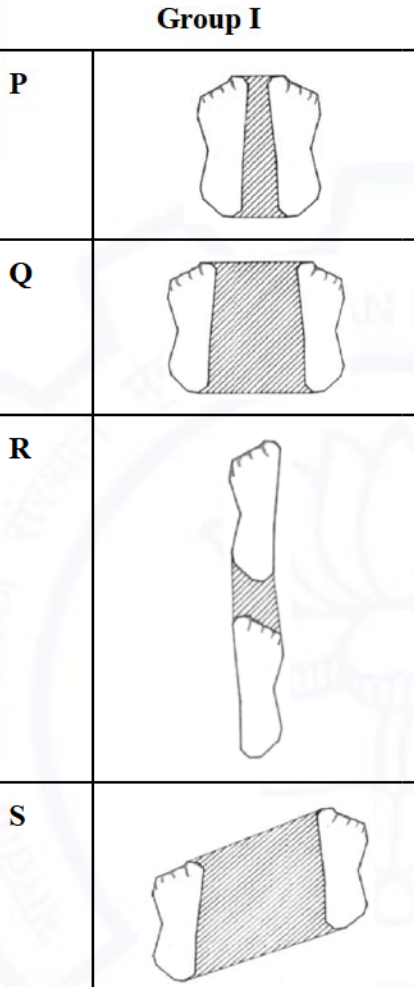
\includegraphics[width=0.25\columnwidth]{figs/10.jpg}
    \caption{Position of Feet}
    \label{fig:Img10}
    \end{figure}
    \newpage
    \textbf{Group II} \\
    1. Stable antero-posteriorly \\
    2. Laterally stable \\
    3. Fairly stable in all directions \\
    4. Vertically stable \\
    5. Unstable \\
    \begin{multicols}{2}
    \begin{enumerate}
        \item P-5, Q-5, R-2, S-1
        \item P-5, Q-3, R-1, S-2
        \item P-1, Q-3, R-4, S-2
        \item P-4, Q-3, R-2, S-1
    \end{enumerate}
    \end{multicols}
    \hfill (GATE-AR 2021)

    \item Match the buildings in \textbf{Group I} with their corresponding structural systems in \textbf{Group II}. \\
    \begin{tabular}{ l l }
    \textbf{Group I} & \textbf{Group II} \\
    P. Empire State Building, New York, USA & 1. Trusses Tube \\
    Q. John Hancock Center, Chicago, USA & 2. Bundled Tube \\
    R. Taipei 101, Taiwan & 3. Tube in Tube \\
    S. Sears Tower, Chicago, USA & 4. Outrigger Frame \\
    & 5. Shear Truss \\
    \end{tabular}
    \begin{multicols}{2}
    \begin{enumerate}
        \item P-5, Q-3, R-4, S-1
        \item P-3, Q-5, R-1, S-2
        \item P-5, Q-4, R-1, S-2
        \item P-5, Q-1, R-4, S-2
    \end{enumerate}
    \end{multicols}
    \hfill (GATE-AR 2021)
    
    \item Choose the correct options with respect to cycle track design as per Indian Road Congress guidelines.
    \begin{enumerate}
    \item The minimum width of cycle track is 3 m if the overtaking is to be provided for
    \item Cycle tracks may be provided when peak hour cycle traffic is 400 or more on routes with a traffic of 100 to 200 vehicles/hour
    \item Maximum gradient allowed for cycle tracks is 1 in 15
    \item Cyclist should have a clear view of at least 80 m
    \end{enumerate}
    \hfill (GATE-AR 2021)
    
    \item As per the Right to Fair Compensation and Transparency in Land Acquisition, Rehabilitation and Resettlement Act, 2013, for which purposes can the urgency clause for land acquisition be invoked?
    \begin{enumerate}
    \item National defence and security purposes
    \item Affordable housing program
    \item Industrial projects
    \item Emergency arising out of natural calamities
    \end{enumerate}
    \hfill (GATE-AR 2021)

    \item Which of the following international treaties are related to Climate Change and global warming?
    \begin{multicols}{2}
    \begin{enumerate}
    \item Cartagena protocol, 2000
    \item Copenhagen summit, 2001
    \item Nagoya protocol, 2010
    \item Paris Agreement, 2016
    \end{enumerate}
    \end{multicols}
    \hfill (GATE-AR 2021)

    \item Which of the following algorithms are used for finding the shortest path in an urban transportation network?
    \begin{multicols}{4}
    \begin{enumerate}
    \item Logit
    \item Huff
    \item Floyd Warshall
    \item Dijkstra
    \end{enumerate}
    \end{multicols}
    \hfill (GATE-AR 2021)

    \item Which of the following statements are true with respect to surface paint?
    \begin{enumerate}
    \item Paint is glossy when Pigment Volume Concentration is high
    \item Vehicle is the volatile part of the paint
    \item Base of the paint is usually oxides of metals
    \item High VOC content is preferred in paints
    \end{enumerate}
    \hfill (GATE-AR 2021)

    \item As per the Solid Waste Management Rules 2016, which among the following are 'Duties of waste generators'?
    \begin{enumerate}
    \item Segregate and store waste generated in four separate streams namely, combustible, non-combustible, organic and domestic hazardous waste
    \item Store construction and demolition waste separately within own premise before disposal
    \item All waste generator shall pay user fee for solid waste management
    \item Compost horticulture waste and garden waste separately within own premise
    \end{enumerate}
    \hfill (GATE-AR 2021)

    \item Choose the correct options with regard to activated sludge process.
    \begin{enumerate}
    \item The activated sludge process is an aerobic process
    \item The entire settled sludge is sent back to the aeration tank
    \item The entire effluent from the final settling tank is sent back to the aeration tank
    \item In aeration tanks, sewage is aerated and agitated for a few hours
    \end{enumerate}
    \hfill (GATE-AR 2021)

    \item A rectangular hall having dimension of 8.0 m $\times$ 14.0 m $\times$ 4.0 m has total 4 windows (1.5 m $\times$ 1.0 m each) and 2 doors (1.0 m $\times$ 2.0 m each). The coefficients of absorption are given below. Considering all windows open and doors closed, the reverberation time in seconds is \rule{2cm}{0.4pt} \\
    \begin{tabular}{ l c }
    Description of item & Absorption coefficient \\
    Coefficient of absorption of wall, floor and ceiling & 0.2 \\
    Coefficient of absorption of door and window & 0.4 \\
    \end{tabular}
    \hfill (GATE-AR 2021)

    \item If surface conductance of external surface is 20 W/m$^2$ \textdegree C, absorbance of the surface is 0.66 and U value of the wall is 1.2 W/m$^2$ \textdegree C, the solar gain factor of a wall is \rule{2cm}{0.4pt}. [round off to 2 decimal places] \\
    \hfill (GATE-AR 2021)

    \item The initial cost of a property is INR 4,00,000 and its future life is 30 years. Considering the scrap value as 10\% of its initial cost and rate of interest as 5\%, the sinking fund (deposited at the end of year) for the property is INR \rule{2cm}{0.4pt}. [round off to 2 decimal places] \\
    \hfill (GATE-AR 2021)

    \item Reading in the staff stationed at P measured by a dumpy level is 3.5 m. The dumpy level is stationed at Q. The Reference Level (RL) at point P is 96.5 m and the height of the dumpy level is 1.25 m. The RL at point Q is \rule{2cm}{0.4pt} m. [round off to 2 decimal places] \\
    \begin{figure}[h!]
    \centering
    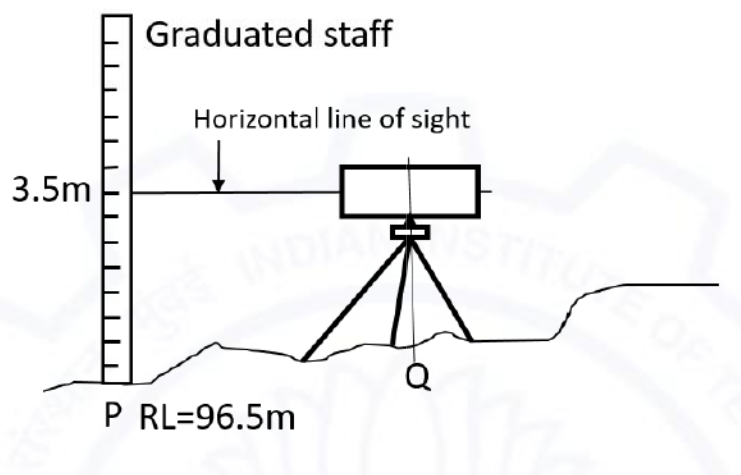
\includegraphics[width=0.5\columnwidth]{figs/11.jpg}
    \caption{Staff}
    \label{fig:Img11}
    \end{figure}
    \hfill (GATE-AR 2021)

    \item A circular cricket field of 180 m diameter is illuminated by four floodlight towers. The floodlight towers are equally spaced along the perimeter of the field. The height of the floodlight tower is 48 m. Using 'Inverse Square Law', the illumination level at the center of the field is found as 750 Lux. Each tower is consisting of 50 lamps. The rating of each lamp is 700 Watt. The efficacy of each lamp is \rule{2cm}{0.4pt} Lumen/Watt. [round off to 2 decimal places] \\
    \hfill (GATE-AR 2021)

    \item A building is constructed on a plot measuring 70 m $\times$ 40 m. The utilized FAR of the building is 1.5. An energy audit team found that the average monthly electricity bill of the building is INR 2,94,000. The unit cost of the electricity is INR 7. The Building Energy Index is \rule{2cm}{0.4pt} kW-hr/m$^2$/year. [in integer] \\
    \hfill (GATE-AR 2021)

    \item A simply-supported steel beam made of an I-section has a span of 8 m. The beam is carrying a uniformly distributed load of 15 kN/m. The overall depth of the beam is 450 mm. The moment of inertia of the beam section is 18000 cm$^4$. The maximum bending stress in the beam will be \rule{2cm}{0.4pt} N/mm$^2$. [in integer] \\
    \hfill (GATE-AR 2021)

    \item The slenderness ratio of a circular column of diameter 300 mm and effective height 3 m is \rule{2cm}{0.4pt}. [in integer] \\
    \hfill (GATE-AR 2021)

    \item A construction project consists of following five activities. The immediate successor activity relationship and duration of each activity are mentioned in the table below. The total duration of the project is \rule{2cm}{0.4pt} weeks. [in integer] \\
    \begin{tabular}{ | c | c | c | }
    \hline
    Activity & Immediate Successor Activity & Duration (Weeks) \\
    \hline
    P & R & 2 \\
    \hline
    Q & R and S & 4 \\
    \hline
    R & T & 5 \\
    \hline
    S & - & 6 \\
    \hline
    T & - & 3 \\
    \hline
    \end{tabular}
    \hfill (GATE-AR 2021)

    \item It is proposed to have ceramic tile flooring in a room having internal clear dimension of 1.8 m $\times$ 2.4 m. Tile sizes are 300 mm $\times$ 300 mm. The door opening is 900 mm and the door is flushed with the internal face of the wall. The height of skirting is 600 mm. The number of ceramic tiles required for internal flooring and skirting is \rule{2cm}{0.4pt}. [in integer] \\
    \hfill (GATE-AR 2021)

    \item In a housing project, 75\% of the permissible FAR was utilised after constructing four numbers eight storey MIG towers with identical floor area of 400 sqm. If three numbers seven storey LIG towers with identical floor area are built utilising the remaining FAR, the floor area of each LIG tower is \rule{2cm}{0.4pt} sqm. [round off to 2 decimal places] \\
    \hfill (GATE-AR 2021)

    \item Using the following values of thermal conductance, surface conductance and thermal resistance, the U value across the given wall cross-section is \rule{2cm}{0.4pt} W/(m$^2$ \textdegree C). [round off to 2 decimal places] \\
    \begin{figure}[h!]
    \centering
    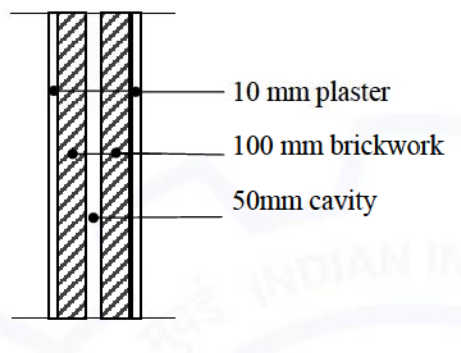
\includegraphics[width=0.5\columnwidth]{figs/12.jpg}
    \caption{Cross-section}
    \label{fig:Img12}
    \end{figure}
    \newpage
    Thermal conductance - \\
    \begin{itemize}
    \item Brick wall 1.2 W/(m \textdegree C)
    \item Plastering 0.5 W/(m \textdegree C)
    \end{itemize}
    Surface conductance - \\
    \begin{itemize}
    \item Internal surface 8.0 W/m$^2$ \textdegree C
    \item External surface 9.5 W/m$^2$ \textdegree C
    \end{itemize}
    Thermal resistance - \\
    \begin{itemize}
    \item 50mm wall cavity 0.17 m$^2$ \textdegree C/W
    \end{itemize}
    \hfill (GATE-AR 2021)
    
\end{enumerate}

\centering
\section*{END OF THE QUESTION PAPER}

\end{document}
